\chapter{Генерация вихревого движения гравитационными волнами} \label{chapt4}
%abstract
В предыдущей главе было показано, что капиллярные волны распространяющиеся под углом друг к другу могут генерировать вихревое движение на поверхности жидкости. Так же было показано, что экспериментальные результаты хорошо согласуются с теоретическими предсказаниями. Стоит заметить, что теоретические построения, объясняющие появление шахматноподобного распределения вихревого поля, пригодны как для капиллярных, так и для гравитационных волн. В этой главе представлены экспериментальные доказательства применимость построенной теории к гравитационным волнам. Кроме того, экспериментально была обнаружена передача энергии вихревого движения из области накачки в большие масштабы.
%Экспериментально исследована генерация вихревого движения на поверхности воды гравитационными волнами на частотах 3 и 4Гц с длиной волны 17 и 9.7 см, соответственно. Показано, что полученные результаты можно описать в рамках модели формирования завихренности нелинейными волнами. Впервые показано, что амплитуда завихренности на поверхности воды зависит от разности фаз между волнами, распространяющимися под углом 90◦ друг к другу с периодом равным, 360◦. Наблюдена квадратичная зависимость амплитуды завихренности на поверхности от угловой амплитуды волн. Обнаружена передача энергии вихревого движения из области накачки в большие масштабы.

\section{Экспериментальная методика} \label{sect4_2}
На рисунке \ref{img:setup} показана схема установки, предназначенной для изучения вихревых и волновых движений на поверхности воды в диапазоне длин волн от 0.25 до 20 см. Ванна изготовлена из оргстекла толщиной 10 мм. Длина ванны равна 140 см, ширина – 70 см, высота – 25 см. Ребра ванны и верхние борта усилены металлическими уголками для придания конструкции жесткости во избежание развития низкочастотных колебаний при работе волнопродукторов. Ванна разделена съемной перегородкой пополам. В данных экспериментах использовалась половина ванны размерами
70 $\times$ 70 см$^2$. Сверху ванна закрывается прозрачным стеклом во избежание попадания на поверхность воды пыли из воздуха. 

\begin{figure}[ht] 
  \center
  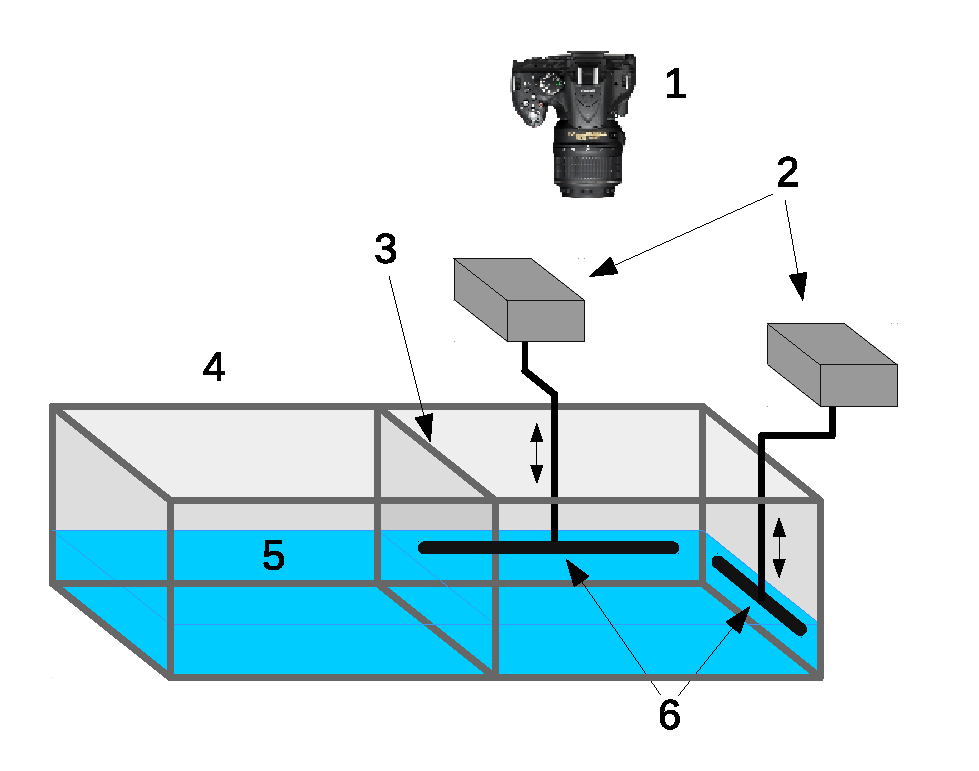
\includegraphics [scale=0.5] {article5/pic_01.eps}
  \caption{Схема установки: 1 – фотоаппарат, 2 – приводы плунжеров, 3 – перегородка, 4 – ванна, 5 – вода, 6 – плунжеры.} 
  \label{img:setup}  
\end{figure}

Ванна установлена на виброизолирующем столе Standa с пневматической подвеской. В ванну, как правило, заливается около 70 л очищенной дистиллированной воды. Глубина воды в ванне составляет около 10 см. Волнопродукторы, состоящие из привода 2 и плунжера 6, монтируются на рамную конструкцию и устанавливаются на столе Standa. Волны на поверхности воды возбуждаются плунжером – трубкой из нержавеющей стали диаметром 10 мм, полупогруженной в воду и совершающей вертикальные колебания. Длина трубки равняется 68 см. Расстояние от трубки до стенки ванны равно 1 см. В качестве привода волнопродукторов применяются сабвуферы TS-W254R фирмы Pioneer номинальной мощностью 250 Вт. Синусоидальные сигналы задаются двухканальным генератором Agilemt 33522B, усиливаются и подаются на сабвуферы. В эксперименте разность фаз $\psi$ сигналов в каналах контролируется. Амплитуда волн, распространяющихся от плунжеров, измеряется в центре ванны с помощью лазерного луча отражающегося от поверхности. Для визуализации движения жидкости на поверхность воды насыпается порошок полиамида белого цвета со средним диаметром гранул около 30 мкм. Частицы полиамида на поверхности воды образуют плоские кластеры с характерным размером 1-3 мм. Плотность образующихся кластеров немного меньше плотности воды, так что они находятся в погруженном состоянии. Поэтому полагаем, что частицы полностью увлекаются потоками жидкости. Частички на поверхности подсвечиваются светодиодами, расположенными по периметру ванны. Видеозапись колеблющейся поверхности производится фотоаппаратом Canon EOS 70D в течение 60 с с частотой 24 кадра/c. Такая частота съемки позволяет выбрать снимки колеблющейся поверхности, находящейся в одной фазе волны. Например, при частоте возбуждающей силы, равной 3 Гц во временном отрезке длительностью 10 с получается 30 последовательных снимков, когда волны возбуждения на поверхности имеют одинаковые фазы. Такой отбор снимков позволяет исключить из дальнейшей обработки осциллирующую составляющую перемещения пробной частицы, плавающей на поверхности. Для выявления треков движения частиц на поверхности снимки суммируются \cite{F8}.

Обработка полученных исходных снимков программой PIVLab \cite{PIVlab, PIVlab1} позволяет вычислить скорости движения частиц $V_x$ и $V_y$, а затем рассчитать завихренность на поверхности по формуле (\ref{eq:defVort}). Распределение энергии по модулю волновых векторов вычисляется усреднением энергии по кольцу в пространстве по формуле:
\begin{equation}
E(k) = \frac{1}{ 2 S \Delta k}\int \frac{d^2 q}{(2 \pi)^2} \lfloor |V_k|^2 \rfloor,
\end{equation}
где интегрирование производится по кольцу от ${k}$ до ${k} + \Delta{k}$. Полученное значение нормируется на площадь поверхности жидкости S. Здесь $V_k$ - Фурье компонента скорости жидкости. Скобки $\lfloor \, \rfloor$ означают усреднение по снимкам, сделанным в разные моменты времени.
	
Групповая скорость волны на частоте 3\,Гц равняется 25\,см/с. Поэтому после включения накачки до возникновения стоячей волны на поверхности воды бегущая волна проходит удвоенное расстояние плунжер-стенка равное 136\,см за 5.5\,с. В представленных ниже результатах мы производили вычисления распределения завихренности и распределения энергии по данным, полученным спустя 15 секунд после включения накачки в интервале длительностью в 5 секунд, чтобы быть уверенным, что амплитуды стоячих волн и завихренность достигли стационарного состояния. Как показывает наши измерения, на временах больше 30 секунд после включения накачки модуль завихренности начинает незначительно уменьшаться. 



\section{Экспериментальные результаты} \label{sect4_3}
На рис. \ref{img:vort_3Hz}а показаны треки полиамидных частиц при накачке поверхности воды на частоте 3\,Гц. При умеренных амплитудах накачки на поверхности хорошо видна решетка из вертикальных и горизонтальных рядов вихрей, аналогичная приведенной в работе \cite{VonKameke2011}. Скорость движения полиамидных частиц составляет в среднем 0.02\,см/с. На рис. \ref{img:vort_3Hz}a показана картина, усредненная по времени в интервале 10 секунд, начиная с 15 секунды после включения накачки.


На рис. \ref{img:vort_3Hz}б показано распределение завихренности, полученное обработкой последовательных изображений программой PIVLab. Хорошо видно, что сформированная в ванне решетка, состоит из малых вихрей близкого размера и с противоположными завихренностями. Периоды решетки в $X$ и $Y$ направлениях составляют 17.5\,см и равняются длине стоячей волны, которая возникла при накачке на частоте 3\,Гц. Суммарная завихренность на поверхности ванны равняется нулю. 

\begin{figure}[ht]
  \begin{minipage}[ht]{0.49\linewidth}
    \center{\includegraphics[width=.82\linewidth]{article5/pic_02a.eps} \\ а)}
  \end{minipage}
  \hfill
  \begin{minipage}[ht]{0.49\linewidth}
    \center{\includegraphics[width=1\linewidth]{article5/pic_02b.eps} \\ б)}
  \end{minipage}
  \caption{а) Треки полиамидных частиц на поверхности воды при накачке двумя плунжерами на частоте 3\,Гц с угловой амплитудой волны в центре ванны $\mu = 0.035$ рад. Плунжеры расположены внизу рисунка и справа. б) Распределение завихренности на поверхности воды при накачке двумя плунжерами на частоте 3\,Гц. Разность фаз $\psi = 90^\circ$.}
  \label{img:vort_3Hz}  
\end{figure}


С повышением уровня накачки амплитуда завихренности каждого вихря на поверхности воды возрастает. На рис.3a показана зависимость корня квадратного из усредненной амплитуды вихрей $\sqrt{\Omega_0}$ на поверхности воды от угловой амплитуды стоячей волны, измеренной в центре ванны. Разность фаз сигналов, подаваемых на плунжеры, $\psi$ равняется $90^\circ$. Хорошо видно, что амплитуда завихренности растет с повышением амплитуды волн по квадратичному закону в соответствии с формулой (\ref{eq:vortStand}). 

На рис. \ref{img:ampl_phase}б показана зависимость амплитуды завихренности на поверхности воды от разности фаз $\psi$ гармонических сигналов, подаваемых на плунжеры на частоте 3\,Гц. Видно, что экспериментальные точки в интервале углов от $0^\circ$ до $180^\circ$ хорошо описываются зависимостью пропорциональной $sin(\psi)$. При изменении разности фаз $\psi$ с $90^\circ$ на $-90^\circ$ амплитуда завихренности сохраняется, но изменяются направления завихренности вихрей в решетке на противоположные. Таким образом, период зависимости $\Omega (\psi)$ равняется $360^\circ$. 

\begin{figure}[ht]
  \begin{minipage}[ht]{0.49\linewidth}
    \center{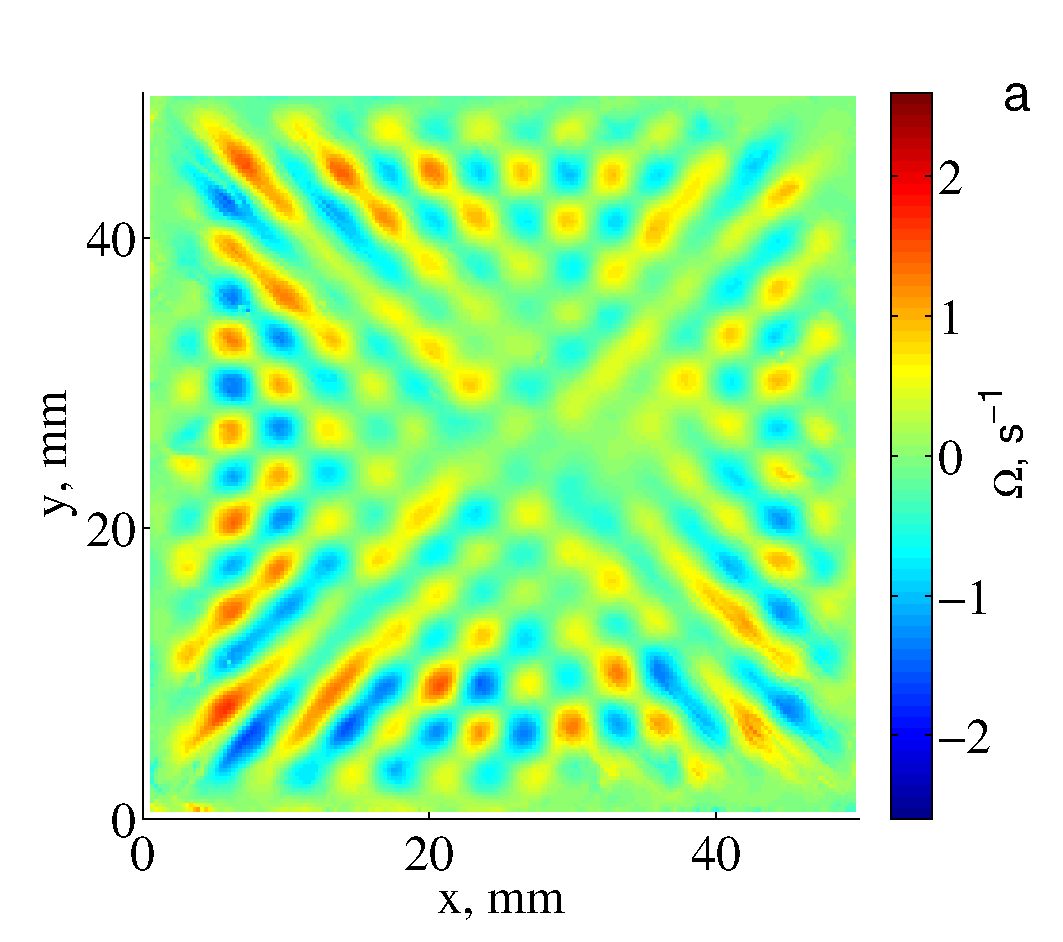
\includegraphics[width=1\linewidth]{article5/pic_03a.eps} \\ а)}
  \end{minipage}
  \hfill
  \begin{minipage}[ht]{0.49\linewidth}
    \center{\includegraphics[width=1\linewidth]{article5/pic_03b.eps} \\ б)}
  \end{minipage}
  \caption{а) Зависимость корня квадратного амплитуды завихренности $\sqrt{\Omega_0}$ на поверхности воды от угловой амплитуды волн $\mu$ при накачке двумя плунжерами на частоте 3\,Гц. Разность фаз $\psi=90^\circ$. б) Зависимость амплитуды завихренности $\Omega_0$ от разности фаз между синусоидальными сигналами, подаваемыми на волнопродукторы. Точки – эксперимент, сплошная кривая $\Omega_0 = \,0.183\, sin(\psi)$}
  \label{img:ampl_phase}  
\end{figure}


При высоком уровне накачки картина треков усложняется: сразу после включения на поверхности формируется решетка вихрей, а затем через время порядка минуты на поверхности развиваются структуры с размерами, превосходящими длину волны накачки. Траектории частиц (треки) со временем медленно изменяются, вихри "дышат". 

На рис. \ref{img:ampl_phase}а приведены треки полиамидных частиц на поверхности воды при накачке двумя плунжерами на частоте 4\,Гц, полученные усреднением в течение 15 секунд через 3 минуты после включения накачки. Амплитуда волн, измеренная на расстоянии 3\,см от плунжеров, равняется $1.0\pm0.2$\,мм. На рисунке хорошо видны два сформировавшихся вихря с характерными размерами близкими к 70\,см (длина стороны ванны), а также вихри меньших размеров. Разность фаз при измерении составляла $\psi$ = $120^\circ$. 

На рис. \ref{img:ampl_phase}б показана вихревая структура, генерируемая стоячими волнами с частотой равной 4\,Гц. Вдоль сторон ванны укладывается по семь длин волн, т.е. длина волны на частоте накачки равна 9.7\,см. Хорошо видна решетка вихрей, немного искажаемая двумя большими вихрями, в нижней и верхней частях рисунка. Суммарная завихренность равна нулю. На рис.5 представлена зависимость модуля полной завихренности $|\Omega|$ на поверхности воды, возбуждаемой двумя плунжерами на частоте 4\,Гц, от фазы $\psi$ между колебаниями плунжеров. 

\begin{figure}[ht]
  \begin{minipage}[ht]{0.49\linewidth}
    \center{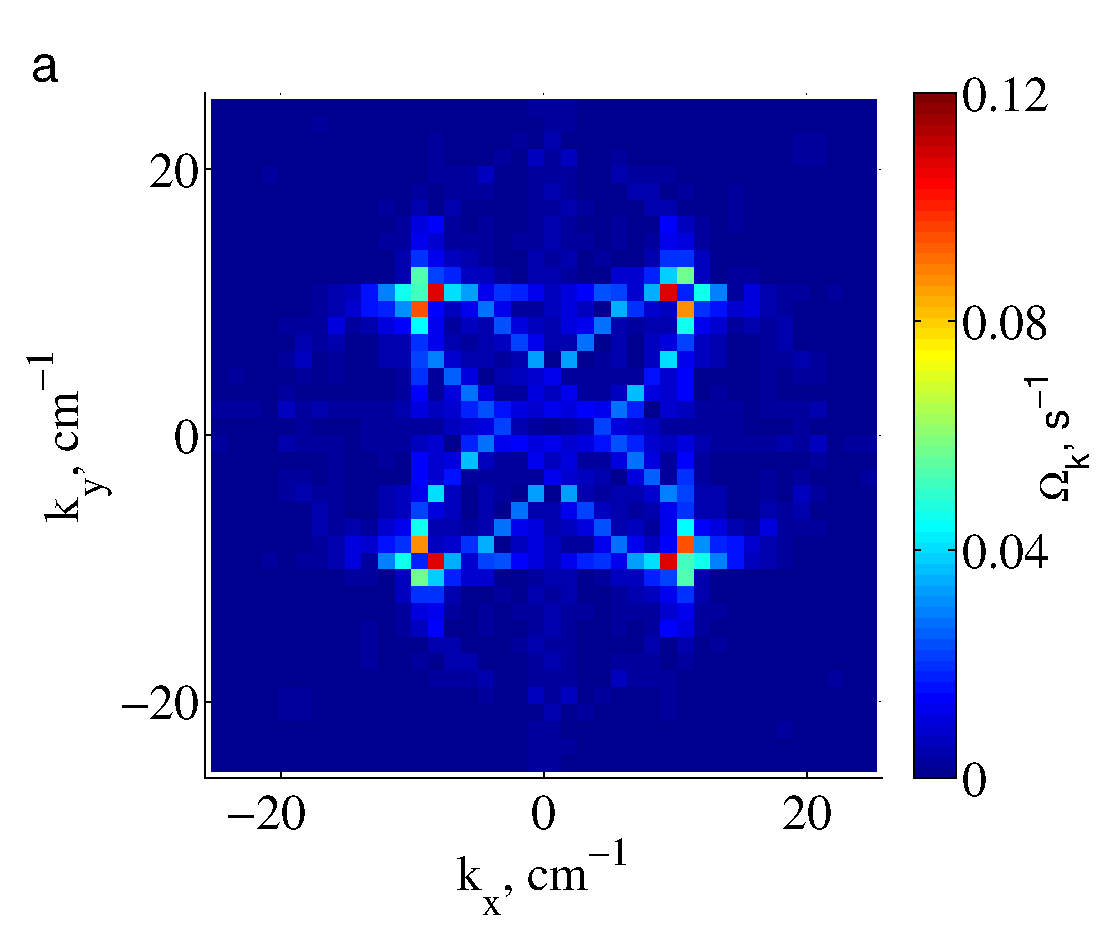
\includegraphics[width=.85\linewidth]{article5/pic_04a.eps} \\ а)}
  \end{minipage}
  \hfill
  \begin{minipage}[ht]{0.49\linewidth}
    \center{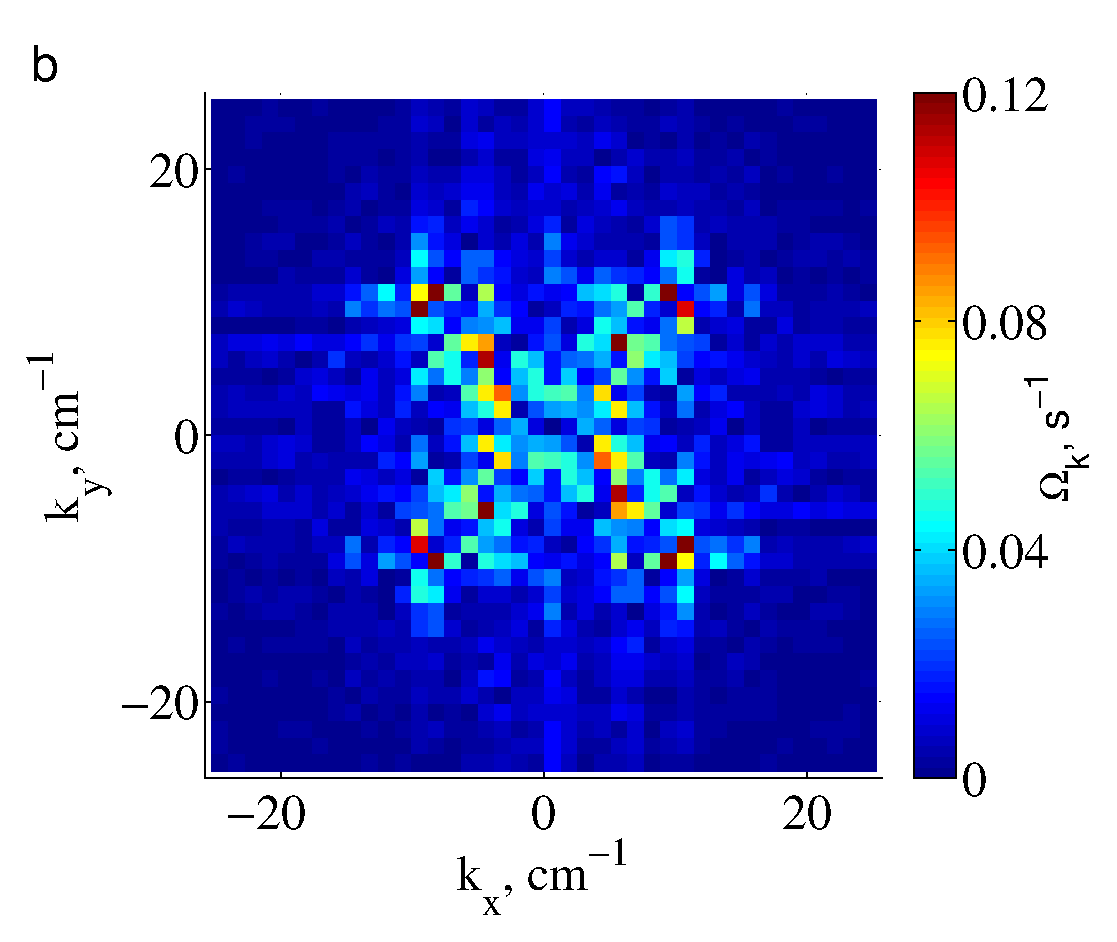
\includegraphics[width=1\linewidth]{article5/pic_04b.eps} \\ б)}
  \end{minipage}
  \caption{а) Треки полиамидных частиц на поверхности воды при накачке двумя плунжерами на частоте 4\,Гц. Амплитуда волн на расстоянии 3\,см от плунжеров равна $H = 1.0 \pm 0.2$\,мм. Плунжеры расположены внизу рисунка и справа. б) Распределение завихренности на поверхности воды. Разность фаз $\psi=120^\circ$.}
  \label{img:vort_4Hz}  
\end{figure}

Начальная разность фаз между колебаниями плунжеров равняется $-30^\circ$. Максимум модуля завихренности наблюдается при $\psi = 120^\circ$ , а минимум – при $\psi = 30^\circ$. Кроме того, очевидно, что в зависимости $|\Omega(\psi)|$ имеется постоянная составляющая, близкая к 0.08\,с$^{-1}$.

Как видно из рис. \ref{img:vort_4Hz} при интенсивной и длительной накачке кроме решетки малых вихрей на поверхности воды возникают вихри больших размеров. Это означает, что в k-пространстве завихренность $\Omega$ и энергия $E$ распространяются из области накачки $\lambda=9.7$\,см на большие масштабы. 
\begin{figure}[ht] 
  \center
  \includegraphics [scale=0.5] {article5/pic_05.eps}
  \caption{Зависимость модуля завихренности на поверхности воды от разности фаз $\psi$ между колебаниями плунжеров на частоте 4\,Гц. Амплитуда волны на расстоянии 3\,см от плунжеров равна $H = 1.0 \pm 0.2$\,мм.} 
  \label{img:phase_4Hz}  
\end{figure}

Результаты вычислений $E(k)$ для вихревых структур, представленных на рис. \ref{img:vort_3Hz} и \ref{img:vort_4Hz}, приведены на рис. \ref{img:spectra} (кривые 1 и 2). Видно, что зависимость $E(k)$ имеет немонотонный характер. В случае возбуждения поверхности волнами на частоте 3\,Гц наблюдается ярко выраженный пик при значении вектора $k = 0.50$\,см$^{-1}$, соответствующего волновому вектору волны накачки. Кроме того, виден пик при значении вектора $k$ равным 1.12\,см$^{-1}$. По-видимому, этот пик может быть связан с формированием завихренности в результате взаимодействия волны генерируемой на частоте накачки и перпендикулярной волны с волновым вектором 1.06\,см$^{-1}$(длина этой волны втрое короче длины волны накачки). Передача энергии в большие масштабы не наблюдается.
\begin{figure}[ht] 
  \center
  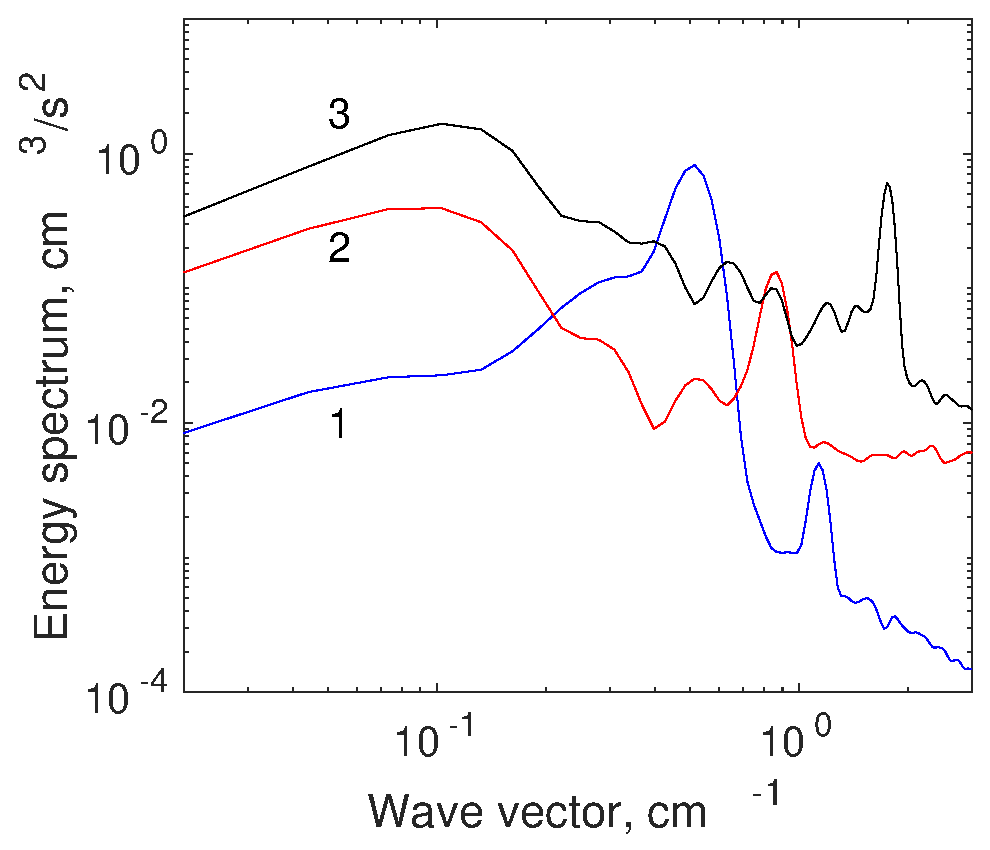
\includegraphics [scale=0.5] {article5/pic_06.eps}
  \caption{Распределение энергии $E(k)$ по волновому вектору при накачке двумя плунжерами на частоте 3\,Гц (кривая 1), 4\,Гц (кривая 2) и 6\,Гц (кривая 3).} 
  \label{img:spectra}  
\end{figure}
Однако в случае накачки на частоте 4\,Гц (рис. \ref{img:spectra}, кривая 2) и формирования на поверхности вихревых структур с размерами больше, чем масштаб накачки, энергия $E(k)$ распределена в интервале волновых векторов от области накачки $k \approx 0.85$\,см$^{-1}$ до больших масштабов $k \approx 0.09$\,см$^{-1}$.

Первый пик, на волновом векторе $k = 0.85$\,см$^{-1}$ находится на масштабе накачки. Эта энергия сосредоточена в малых вихрях, которые формируют решетку. Видно, что с уменьшением $k$ наблюдается рост $E(k)$. Максимум распределения $E(k)$ приходится на волновой вектор близкий к 0.09\,см$^{-1}$, который соответствует размерам больших вихрей, сформировавшихся в ванне. Дополнительно на рис. \ref{img:spectra} кривой 3 представлено распределение $E(k)$ при накачке волнами с меньшей длиной волны  (частота 6 Гц, длина волны 4.9 см). На этом распределении также наблюдаются два экстремума, соответствующие масштабу накачки,  $k = 1.8$\,см$^{-1}$  и максимуму энергии,  $k = 0.1$\,см$^{-1}$. Из сравнения распределений 2 и 3 можно заключить, что  масштаб большого вихря не зависит от длины волны накачки и определяется размерами ванны. В области волновых векторов $k > 2\,$см$^{-1}$ значения $E(k)$ более чем на порядок меньше значений амплитуд в основных пиках. Т.е. прямой каскад практически не сформировался: вся энергия уходит на поддержание больших вихрей, где она диссипирует в силу вязких потерь. 

\section{Обсуждение экспериментальных результатов} \label{sect4_4}
Так же как в \cite{F5, F6} в настоящей работе наблюдается решетка из вихрей с периодом равным длине волны накачки. Это свидетельствует о справедливости модели генерации вихрей нелинейными волнами и подтверждает обоснованность применения формул (\ref{eq:vortStand}) и (\ref{eq:vortRun}) для описания завихренности на поверхности жидкости в широком диапазоне длин волн: от 0.5\,см до 17\,см. Следует отметить, что при накачке на частоте 3\,Гц решетка вихрей (рис. \ref{img:vort_3Hz}) является столь же совершенной, как и при накачке капиллярными волнами \cite{F6}, где измерения проводились в специальном боксе с чистой атмосферой. В случае гравитационных волн, если ванну не закрывать сверху прозрачным стеклом, то на поверхности чистой воды за время порядка 1 часа формируется тонкая несжимаемая пленка, в результате чего затухание волн значительно возрастает \cite{land}, что отражается на распределении завихренности.

На рис. \ref{img:vort_3Hz}б и \ref{img:vort_4Hz}б, где приведены решетки вихрей, затухание волны не является существенным. Амплитуда отраженной от стенки волны незначительно отличается от амплитуды волны идущей навстречу от плунжера. Согласно формулам (\ref{eq:vortStand}) и (\ref{eq:vortRun}) отличия в этих амплитудах не должны отражаться на квадратичной зависимости завихренности от амплитуд волн. 

Фазовая зависимость амплитуды завихренности при возбуждении волн двумя плунжерами на частоте 3\,Гц очень хорошо описывается периодической функцией пропорциональной $sin(\psi)$. Период функции $\Omega (\psi)$ составляет $360^\circ$, как это и следует из зависимости (\ref{eq:vortStand}). 

Несколько более сложная ситуация наблюдается в экспериментах по исследованию зависимости модуля завихренности от разности фаз $\psi$ между двумя перпендикулярными возбуждающими волнами на частоте 4\,Гц. Как сказано выше, на поверхности воды присутствуют как вихри, формирующие решетку, так и вихри большего масштаба, возникшие в силу нелинейного взаимодействия вихрей и волн. Это хорошо видно на рис. \ref{img:vort_4Hz}a, где на поверхности присутствуют как решетка из одиночных вихрей, так и большие вихри. В связи с этим фазовая зависимость завихренности не может описываться формулой (\ref{eq:vortStand}), а должна содержать некоторый член, отражающей присутствие вихрей большего масштаба. Видно, что накачка вихрей не исчезает даже при $\psi=0^\circ$, то есть присутствие крупномасштабных вихревых течений на поверхности усложняет генерацию вихрей нелинейными поверхностными волнами, описываемую простыми зависимостями (\ref{eq:vortStand}) или (\ref{eq:vortRun}). Величина $|\Omega|$ осциллирует около некоторого пьедестала. По результатам проведенных экспериментов нельзя сказать изменяется ли высота этого пьедестала с ростом разности фаз, поэтому в первом приближении полагаем его постоянным. 

Полученный экспериментальный результат качественно не противоречит модели, представленной в \cite{F6}. Как видно из рис. \ref{img:phase_4Hz} зависимость $|\Omega|$ от разности фаз $\psi$ имеет периодический характер с двумя экстремумами. Период равняется $180^\circ$. Таким образом зависимость модуля завихренности $|\Omega|$ от разности фаз можно описать формулой: 

\begin{equation}\label{eq:fit_abs}
|\Omega| = A |sin(\psi+\psi_0)| + \Omega_0
\end{equation}
где $\psi_0$ - начальный сдвиг фаз, $\Omega_0$ – постоянное слагаемое. Из подгонки зависимости (\ref{eq:fit_abs}) к экспериментальным точкам следует что $\psi_0 = -9^\circ$, $\Omega_0$ = 0.077\,с$^{-1}$, A = 0.028\,с$^{-1}$. Отметим, что постоянное слагаемое определяется структурой больших вихрей, возникающих на поверхности и, отличается в разных реализациях эксперимента при одинаковых начальных условиях. 

Отметим, что абсолютные величины модуля завихренности, полученные в экспериментах по измерению зависимостей амплитуды завихренности от амплитуды волн и разности их фаз приблизительно в 4 раза превосходят теоретическую величину, вычисленную по выражению (\ref{eq:vortStand}). Гранулы на поверхности слипаются в более крупные образования с размерами порядка 1 мм.Аналогичное расхождение наблюдалось и в случае капиллярных волн в работе \cite{F6}. 

Так же следует отметить, что при накачке на низких частотах, соответствующих гравитационным волнам, всегда через некоторое время после включения накачки наблюдается формирование структуры (вихрей) с характерным размером больше масштаба накачки. Вихрь может занимать почти всю поверхность ванны, за исключением небольших участков, где располагаются ``смазывающие" вихри, которые обеспечивают нулевую суммарную завихренность, либо их может быть несколько. Отметим также, что при работе с капиллярными волнами большие вихри возникали только после превышения порога параметрической неустойчивости \cite{Francois2013}. 

Как следует из зависимостей, представленных на рис. \ref{img:spectra} (кривые 2 и 3), энергия вихревого движения из области накачки передается в область больших масштабов. Очевидно, что энергия от поверхностных волн поступает сначала в систему вихрей, которые выстроены в решетку. Затем в силу нелинейного взаимодействия энергия распространяется на большие масштабы. Видно, что в основном энергия передается в большие вихри, а в сторону малых масштабов не идет: прямой каскад в сторону больших $k$ (малых масштабов) практически отсутствует.

Обратный каскад наблюдали ранее в экспериментах при генерации фарадеевских волн на поверхности \cite{Francois2014}. Оказалось, что экспериментальное распределение энергии по волновому вектору можно хорошо описать зависимостью $E(k) \sim k^{-5/3}$. Эта зависимость для обратного каскада энергии была предсказана теоретически Крайчнаном \cite{Kraichnan1967} для тонких двумерных слоев жидкости. В случае прямого каскада $E(k) \sim k^{-3}$ \cite{Kraichnan1967}. В наших экспериментах область накачки и область диссипации не разнесены достаточно далеко в k-пространстве, чтобы сформировался развитый каскад, описываемый степенной функцией $k$.

Подчеркнем, что в наших экспериментах мы имеем дело с трехмерным случаем, так как глубина ванны больше глубины проникновения волн на всех используемых частотах накачки. Однако передача энергии из области накачки в большие масштабы, свойственная двумерному случаю, определенно наблюдается. 

Расхождения по абсолютной величине завихренности с теоретической оценкой и формирование обратного каскада, свойственного двумерным системам, в наших трехмерных экспериментах требуют дополнительных экспериментальных и теоретических исследований.

\section{Выводы} \label{sect4_5}
В данной работе впервые экспериментально показано, что завихренность, формируемая на поверхности воды слабо нелинейными гравитационными волнами, зависит от разности их фаз и хорошо описывается выражениями, полученными в работе \cite{F6}. Амплитуда завихренности на поверхности квадратично зависит от амплитуды волн. Таким образом, модель генерации вихревого движения нелинейными волнами применима для описания завихренности на поверхности жидкости не только для волн капиллярного диапазона с длиной волны около 0.5\,см, но и для гравитационных волн с длинами волн порядка 10\,см. 
Экспериментально наблюдена передача энергии из области накачки (масштаб решетки вихрей) в область больших масштабов. Механизм передачи энергии пока неустановлен, требуются дополнительные исследования.
%Так же наблюдена передача энергии от слабонелинейного волнового движения в систему вихрей, образующих решетку, с последующей передачей в большие масштабы.


%\section{Генерация вихревого движения гравитационными волнами} \label{sect4_3}

\clearpage